% Provenance (never printed): see sources/outline_sources.md (Year 2: interstellar
% medium, molecular clouds, gravitational collapse and the Jeans criterion, protostars
% and protostellar discs). Curves from figdata/bachelor-2/jeans.py; exercise and problem
% values in the Book 4 scratch calculator calc/ch01.py.
\chapter{El medio interestelar y la formación de estrellas}\label{ch:b2:ism-star-formation}

En la constelación de Tauro, a unos \qty{140}{\parsec} del Sol, una mancha
oscura tapa las estrellas que hay detrás. Vista con un radiotelescopio
sintonizado en las líneas del monóxido de carbono, la mancha es una nube de gas
frío de una masa unas veinte mil veces la del Sol, surcada de filamentos;
dentro de sus nudos más densos están naciendo estrellas, y alrededor de una de
ellas, HL Tauri, un disco de polvo muestra un dibujo de anillos brillantes y
oscuros donde quizá ya se estén formando planetas. El Sol, la Tierra y cada
átomo de las rocas de este libro estuvieron una vez en una nube así. Este
capítulo sigue la materia de un sistema planetario desde el gas tenue entre las
estrellas hasta un disco alrededor de una estrella recién nacida: de qué está
hecho el \omterm{def:b2:ism-star-formation:ism}{medio interestelar}, por qué llega a colapsar una nube sostenida por su propio
calor, cuánto dura el colapso, cómo reúne una estrella su masa y por qué la materia que no cae en ella acaba en un disco.

\begin{recall}
Una estrella de la secuencia principal brilla fusionando hidrógeno en helio en
su núcleo y se sostiene por su presión frente a su propio peso; su posición en
el diagrama de Hertzsprung--Russell la fija su masa (física, tercer año
universitario). Un cuerpo en órbita cerrada alrededor de una masa $M$ cumple la
tercera ley de Kepler, $T^2 = 4\pi^2 a^3/(GM)$ (física, primer año
universitario). Un cuerpo negro de temperatura $T$ emite $\sigma T^4$ por unidad
de área (física, segundo año universitario). En un gas ideal de $N$ partículas
la energía cinética media de traslación es $\tfrac32 N k_{\mathrm B} T$. El
pársec, \qty{3.086e16}{m}, es la unidad de distancia del volumen de primer año.
\end{recall}

\section{La materia entre las estrellas}

El espacio entre las estrellas no está vacío. Cerca del Sol contiene en promedio
un átomo de hidrógeno por centímetro cúbico, una densidad de masa de
\qty{2.7e-24}{g.cm^{-3}}; el aire que respiramos contiene unas $10^{19}$ veces
más moléculas en el mismo volumen (\cref{exo:b2:ism-star-formation:1}). Repartida por la Galaxia, esta materia tenue
supone aun así un \qtyrange{10}{15}{\percent} de la masa del
disco galáctico.
% ledger: ferriere:mean-density, ferriere:disc-fraction

\begin{definition}[Medio interestelar, polvo interestelar]
\label{def:b2:ism-star-formation:ism}
El \emph{medio interestelar}\index{medio interestelar} es el gas y el polvo
que llenan el espacio entre las estrellas de una galaxia. El \emph{polvo
interestelar}\index{polvo interestelar} es la parte que está en granos sólidos, de unos
pocos nanómetros a cerca de un micrómetro de tamaño, hechos de silicatos, compuestos
de carbono y, en las regiones frías, hielos.
\end{definition}

Su composición es la que se mide en el Sol y en los meteoritos: en masa,
\qty{70.4}{\percent} de hidrógeno, \qty{28.1}{\percent} de helio y
\qty{1.5}{\percent} de elementos más pesados. Solo un \qtyrange{0.5}{1}{\percent} de la
masa está en el polvo, y sin embargo el polvo retiene la mayor parte de algunos elementos: el gas es
más pobre que el Sol en magnesio, silicio y hierro por factores de 10 a 100, porque
esos átomos están encerrados en los granos, mientras que el carbono, el nitrógeno y el oxígeno
solo están empobrecidos por factores de 1.2 a 3. Los granos son los primeros sólidos de un
futuro sistema planetario; el \cref{ch:b2:planet-formation-meteorites}
los sigue.
% ledger: ferriere:composition, ferriere:dust-fraction, ferriere:refractory-depletion

\subsection{Cinco fases}

El gas dista mucho de ser uniforme. Se presenta en unos pocos estados distintos, o fases,
cada uno con su propio intervalo de temperatura y de densidad (tabla siguiente). Cerca de la mitad
de su masa está en nubes que ocupan solo un \qtyrange{1}{2}{\percent} del volumen;
el resto, templado o caliente, llena el espacio entre ellas.
% ledger: ferriere:disc-fraction

\begin{table}[htbp]
\centering
\small
\begin{tabular}{lll}
\hline
fase & temperatura (K) & densidad $n$ (\unit{cm^{-3}}) \\
\hline
molecular & 10--20 & $10^2$--$10^6$ \\
atómica fría & 50--100 & 20--50 \\
atómica templada & 6000--10\,000 & 0.2--0.5 \\
ionizada templada & unos 8000 & 0.2--0.5 \\
ionizada caliente & unos $10^6$ & unos 0.0065 \\
\hline
\end{tabular}
\caption{Las fases del gas interestelar cerca del Sol; $n$ es la densidad
numérica de núcleos de hidrógeno.}
\label{tab:b2:ism-star-formation:phases}
% ledger: ferriere:molecular, ferriere:cold-atomic, ferriere:warm-atomic, ferriere:warm-ionized, ferriere:hot-ionized
\end{table}

La tabla esconde una regularidad. La presión de un gas ideal es
$P = n k_{\mathrm B} T$, de modo que el producto $nT$ la mide. Para el gas atómico frío
$nT$ vale unos $30\times75 \approx 2000$ (en \unit{K.cm^{-3}}), para el gas atómico
templado unos $0.3\times8000 \approx 2400$, para el gas caliente unos
$0.0065\times10^6 = 6500$: salvo un factor de unas pocas unidades, las tres fases que
comparten el espacio entre las nubes están a la misma presión (figura siguiente).
Donde un gas caliente y uno frío se tocan a igual presión, ninguno empuja al otro;
un gas que se enfría a presión constante se vuelve más denso en proporción y
pasa de la fase templada a la fría. Las \omterm{def:b2:ism-star-formation:molecular-cloud}{nubes moleculares} alcanzan presiones mucho más altas, hasta miles de veces mayores en sus partes densas: las mantiene unidas su propia gravedad, no la
presión de su entorno.

\begin{omfigure}
\begin{tikzpicture}
\begin{axis}[omrecord, width=0.86\linewidth, height=6.4cm, xmode=log, ymode=log,
  xmin=1e-3, xmax=1e7, ymin=3, ymax=3e6,
  xlabel={densidad de núcleos de hidrógeno $n$ (\unit{cm^{-3}})}, ylabel={temperatura $T$ (K)},
  tick label style={font=\scriptsize}, label style={font=\small}, clip=false,
  legend pos=north east, legend style={font=\scriptsize, draw=black!30}]
\addplot[black!45, densely dashed, domain=1e-3:1e3, samples=2] {3000/x};
\addlegendentry{$nT = \num{3000}$}
\addplot[black!60, densely dotted, thick, domain=0.1:1e5, samples=2] {3e5/x};
\addlegendentry{$nT = 3\times10^5$}
\fill[blue!45, opacity=0.6] (axis cs:1e2,10) rectangle (axis cs:1e6,20);
\fill[teal!50, opacity=0.6] (axis cs:20,50) rectangle (axis cs:50,100);
\fill[orange!55, opacity=0.6] (axis cs:0.2,6000) rectangle (axis cs:0.5,10000);
\fill[red!45, opacity=0.6] (axis cs:0.2,5714) rectangle (axis cs:0.5,11200);
\fill[violet!50, opacity=0.6] (axis cs:0.00464,7.14e5) rectangle (axis cs:0.0091,1.4e6);
\node[font=\scriptsize, anchor=south east] at (axis cs:1e6,20) {nubes moleculares};
\node[font=\scriptsize, anchor=south west] at (axis cs:50,100) {atómica fría};
\node[font=\scriptsize, anchor=east, align=right] at (axis cs:0.17,8000) {atómica templada\\e ionizada templada};
\node[font=\scriptsize, anchor=west] at (axis cs:0.011,1e6) {ionizada caliente};
\end{axis}
\end{tikzpicture}

\par\smallskip{\small Las fases del gas interestelar cerca del Sol (intervalos de la tabla
anterior; las fases ionizada templada y caliente, dadas como valores únicos, se dibujan como cajas
de un factor 1.4 de anchura). A lo largo de cada línea gris la presión $nk_{\mathrm B}T$ es constante: las
fases fría, templada y caliente están cerca de la misma presión, salvo un factor de unas pocas unidades,
mientras que las \omterm{def:b2:ism-star-formation:molecular-cloud}{nubes moleculares}, ligadas por su propia gravedad, alcanzan presiones hasta miles de veces mayores.
Datos: Ferrière (2001).}
\end{omfigure}

El polvo se manifiesta de tres maneras. Atenúa la luz de las estrellas que hay detrás,
y atenúa más la luz azul que la roja, de modo que las estrellas vistas a través de él parecen más rojas
de lo que son. Brilla en el infrarrojo lejano y en longitudes de onda milimétricas,
a la temperatura de unas pocas decenas de kelvin a la que lo calienta la luz estelar. Y
oculta a los telescopios ópticos todo lo que hay dentro de una nube densa, razón por la cual
la formación estelar se observa en longitudes de onda de radio e infrarrojas. El gas se
rastrea por sus líneas: el hidrógeno atómico por su línea de radio de \qty{21}{cm},
el hidrógeno molecular, que apenas radia cuando está frío, por las líneas de las
moléculas que lo acompañan, la primera de ellas el monóxido de carbono.

\section{Nubes moleculares}

La fase más fría y densa es donde se forman las estrellas.

\begin{definition}[Nube molecular, núcleo denso]
\label{def:b2:ism-star-formation:molecular-cloud}
Una \emph{nube molecular}\index{nube molecular} es una región del
\omterm{def:b2:ism-star-formation:ism}{medio interestelar} lo bastante densa y opaca para que su hidrógeno esté sobre todo en
moléculas, \ce{H2}, protegidas por el polvo de la luz ultravioleta de las estrellas
que las rompería; su temperatura es de unos \qty{10}{K} a \qty{20}{K}. Un
\emph{núcleo denso}\index{núcleo denso} es una condensación compacta dentro de una
nube molecular, de unas pocas décimas de pársec de diámetro o menos, con densidades de
$10^4$ a $10^5$ partículas por centímetro cúbico, a partir de la cual se forma una sola estrella o un
pequeño grupo de estrellas.
\end{definition}

Las nubes se organizan en una jerarquía (tabla siguiente). Una nube oscura como Tauro
contiene grumos, y los grumos contienen núcleos, cada nivel más denso, más pequeño y más
tranquilo que el anterior: en un núcleo el gas se mueve como mucho a unas pocas décimas de
kilómetro por segundo, la velocidad del sonido en un gas a \qty{10}{K}. La
región de Tauro cartografiada en monóxido de carbono contiene unas \num{2.4e4} masas
solares de gas; solo un \qtyrange{0.3}{1.2}{\percent} se ha convertido en las
estrellas jóvenes que se ven allí, a un ritmo de unas ocho estrellas cada cien mil
años durante los últimos tres millones de años. La formación estelar es lenta y derrochadora.
% ledger: bt07:clouds, bt07:clumps, bt07:cores, goldsmith:taurus-mass, goldsmith:taurus-sfe, goldsmith:taurus-distance

\begin{table}[htbp]
\centering
\small
\begin{tabular}{lccc}
\hline
 & nubes oscuras & grumos & \omterm{def:b2:ism-star-formation:molecular-cloud}{núcleos densos} \\
\hline
masa (masas solares) & $10^3$--$10^4$ & 50--500 & 0.5--5 \\
tamaño (pc) & 2--15 & 0.3--3 & 0.03--0.2 \\
densidad media (\unit{cm^{-3}}) & 50--500 & $10^3$--$10^4$ & $10^4$--$10^5$ \\
temperatura del gas (K) & unos 10 & 10--20 & 8--12 \\
ejemplos & Tauro, Musca & --- & L1544, B68 \\
\hline
\end{tabular}
\caption{La jerarquía de una \omterm{def:b2:ism-star-formation:molecular-cloud}{nube molecular} oscura. Las densidades cuentan todas las
partículas. Datos: Bergin y Tafalla (2007).}
\label{tab:b2:ism-star-formation:hierarchy}
% ledger: bt07:clouds, bt07:clumps, bt07:cores
\end{table}

¿Por qué son tan frías las nubes? El gas pierde energía emitiendo fotones que
escapan, y las moléculas son emisoras eficaces: una colisión eleva una molécula de
monóxido de carbono a un nivel de rotación superior, la molécula vuelve a caer
emitiendo un fotón de longitud de onda milimétrica, y el fotón sale de la nube
llevándose la energía de la colisión. El polvo, calentado por la débil
luz estelar que entra, radia en el infrarrojo lejano. El calentamiento, por los rayos
cósmicos y por la luz estelar filtrada por el polvo, es débil; el balance se estabiliza
cerca de \qty{10}{K}. En un gas así la presión térmica es pequeña, y la gravedad puede
imponerse.

\begin{omfigure}
\begin{minipage}[c]{0.44\linewidth}
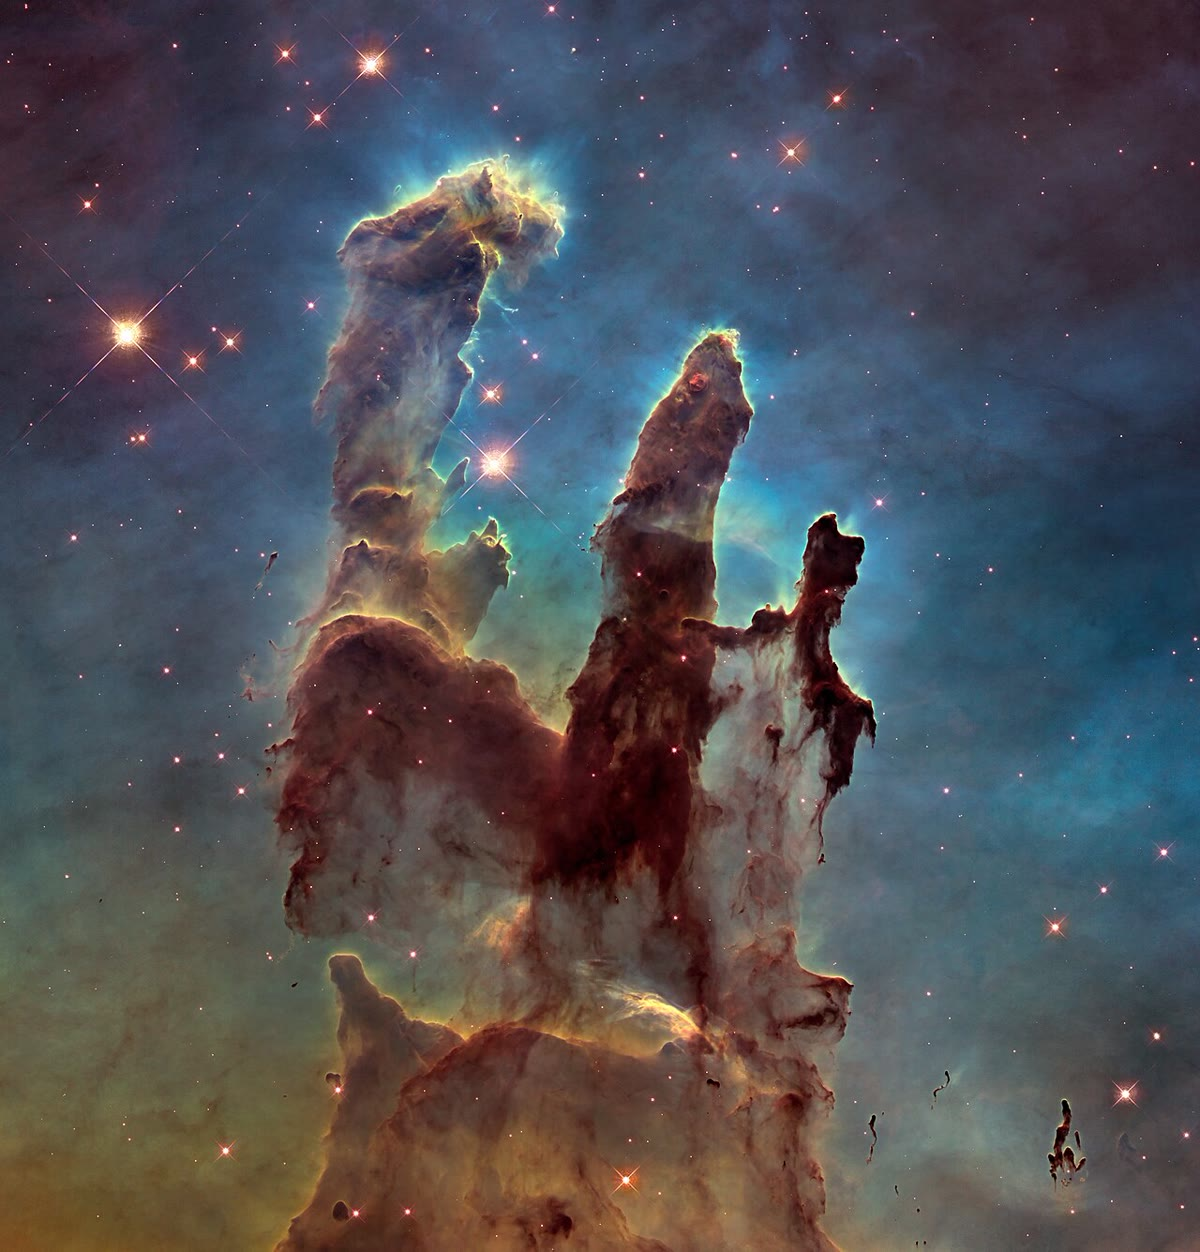
\includegraphics[width=\linewidth]{images/book4/b2-pillars-of-creation.jpg}
\end{minipage}\hfill
\begin{minipage}[c]{0.52\linewidth}
{\small Los «Pilares de la Creación» de la nebulosa del Águila, fotografiados por el
telescopio espacial Hubble en luz visible. Las columnas son gas molecular frío y denso y
polvo, de años luz de longitud, erosionadas e iluminadas desde arriba por la luz ultravioleta de
estrellas jóvenes masivas fuera de la imagen; el polvo las hace opacas. Pequeñas
condensaciones en sus extremos están formando estrellas. NASA, ESA y el Hubble
Heritage Team (STScI/AURA), dominio público.}
\end{minipage}
\end{omfigure}

\section{El colapso gravitatorio}

Una nube es un equilibrio entre dos energías: la energía térmica de su gas,
que empuja hacia fuera, y su energía gravitatoria, que tira hacia dentro. La
segunda crece con la masa más deprisa que la primera; por encima de cierta masa, la gravedad
se impone.

\begin{proposition}[Energía gravitatoria de una esfera uniforme]
\label{prop:b2:ism-star-formation:grav-energy}
Una esfera de densidad uniforme, de masa $M$ y radio $R$, tiene la
energía potencial gravitatoria
\[
  U = -\frac{3}{5}\,\frac{G M^2}{R}.
\]
\end{proposition}

\begin{proof}
Constrúyase la esfera capa a capa. Cuando su radio es $r$ tiene la masa
$m(r) = M r^3/R^3$; traer una capa de espesor $\mathrm dr$, de masa
$\mathrm dm = 3M r^2\,\mathrm dr/R^3$, desde el infinito hasta su superficie libera
la energía $G m(r)\,\mathrm dm/r$, porque una esfera atrae hacia fuera como si
su masa estuviera en su centro (el teorema de las capas, física). Por tanto
\[
  U = -\int_0^R \frac{G}{r}\,\frac{M r^3}{R^3}\,\frac{3 M r^2}{R^3}\,\mathrm dr
    = -\frac{3 G M^2}{R^6}\int_0^R r^4\,\mathrm dr = -\frac{3}{5}\,\frac{G M^2}{R}.
  \qedhere
\]
\end{proof}

Un cuerpo autogravitante en equilibrio cumple el teorema del virial: en promedio
temporal, el doble de su energía cinética más su energía gravitatoria es cero,
$2K + U = 0$ (física, tercer año universitario, donde se deduce de las
ecuaciones del movimiento). Para una nube en reposo, $K$ es la energía térmica de sus
partículas. Si $2K > |U|$ el gas se expande; si $2K < |U|$ la gravedad no tiene
equilibrio que la contrarreste y la nube se contrae.

\begin{proposition}[Criterio de Jeans]\label{prop:b2:ism-star-formation:jeans}
Una nube uniforme e isoterma de temperatura $T$ y densidad $\rho$, formada por
partículas de masa media $\mu m_u$, colapsa bajo su propia gravedad si su masa
supera la \emph{\omterm{def:b2:ism-star-formation:jeans}{masa de Jeans}}
\[
  M_J = \left(\frac{5 k_{\mathrm B} T}{G\mu m_u}\right)^{3/2}
        \left(\frac{3}{4\pi\rho}\right)^{1/2},
\]
o, de forma equivalente, si su radio supera la \emph{\omterm{def:b2:ism-star-formation:jeans}{longitud de Jeans}}
\[
  R_J = \left(\frac{15 k_{\mathrm B} T}{4\pi G\mu m_u\,\rho}\right)^{1/2}.
\]
Este es el \emph{criterio de Jeans}\index{criterio de Jeans}.
\end{proposition}

\begin{proof}
La nube contiene $N = M/(\mu m_u)$ partículas, con la energía térmica
$K = \tfrac32 N k_{\mathrm B}T = \tfrac32 M k_{\mathrm B}T/(\mu m_u)$. Por la
\cref{prop:b2:ism-star-formation:grav-energy}, colapsa si
$2K < \tfrac35 GM^2/R$, es decir
\[
  \frac{3 M k_{\mathrm B} T}{\mu m_u} < \frac{3}{5}\,\frac{G M^2}{R}
  \iff M > \frac{5 k_{\mathrm B} T}{G \mu m_u}\, R .
\]
Elimínese $R$ con $M = \tfrac43\pi R^3\rho$, es decir $R = (3M/4\pi\rho)^{1/3}$:
$M^{2/3} > \frac{5 k_{\mathrm B}T}{G\mu m_u}\,(3/4\pi\rho)^{1/3}$, y elevando
ambos miembros a la potencia $3/2$ se obtiene $M > M_J$. Eliminando en cambio $M$,
$\tfrac43\pi R^3\rho > 5 k_{\mathrm B}T R/(G\mu m_u)$ da $R^2 > 15
k_{\mathrm B}T/(4\pi G\mu m_u\rho)$, es decir $R > R_J$.
\end{proof}

\begin{definition}[Masa de Jeans, longitud de Jeans]\label{def:b2:ism-star-formation:jeans}
La \emph{masa de Jeans}\index{masa de Jeans} $M_J$ y la \emph{longitud
de Jeans}\index{longitud de Jeans} $R_J$ de un gas de temperatura y densidad dadas
son la masa y el radio por encima de los cuales una esfera uniforme de ese gas
colapsa bajo su propia gravedad (\cref{prop:b2:ism-star-formation:jeans}).
\end{definition}

La \omterm{def:b2:ism-star-formation:jeans}{masa de Jeans} crece como $T^{3/2}$ y disminuye como $\rho^{-1/2}$: el gas frío y denso
es el que colapsa con más facilidad. En una \omterm{def:b2:ism-star-formation:molecular-cloud}{nube molecular} la masa media por partícula es
$\mu = 2.33$ unidades de masa atómica, hidrógeno molecular con un átomo de helio por
cada cinco moléculas aproximadamente. A \qty{10}{K} y $10^4$ partículas por centímetro
cúbico, $\rho = \mu m_u n = \qty{3.87e-17}{kg.m^{-3}}$ y
$M_J = 5.5$ masas solares, dentro de una \omterm{def:b2:ism-star-formation:jeans}{longitud de Jeans} de \qty{0.13}{\parsec}:
la masa y el tamaño de un \omterm{def:b2:ism-star-formation:molecular-cloud}{núcleo denso}. A la densidad media de una nube oscura,
$100$ partículas por centímetro cúbico, la \omterm{def:b2:ism-star-formation:jeans}{masa de Jeans} es diez veces mayor, 55
masas solares, y una nube de \num{24000} masas solares como Tauro contiene
cientos de ellas (figura siguiente).
% ledger: kauffmann:mu, nist:u, const:kB, const:G, sun:mass, goldsmith:taurus-mass

\begin{omfigure}
\begin{tabular}{@{}c@{\hspace{3mm}}c@{}}
\begin{tikzpicture}
\begin{axis}[omrecord, width=0.455\linewidth, height=6.0cm, xmode=log, ymode=log,
  xmin=10, xmax=1e7, ymin=0.05, ymax=1e4,
  xlabel={$n$ (\unit{cm^{-3}})}, ylabel={masa de Jeans (masas solares)},
  tick label style={font=\scriptsize}, label style={font=\small},
  legend style={font=\scriptsize, at={(0.97,0.97)}, anchor=north east, draw=none, fill=white, fill opacity=0.85}]
\fill[blue!12] (axis cs:1e4,0.5) rectangle (axis cs:1e5,5);
\node[font=\scriptsize, blue!50!black, anchor=north east] at (axis cs:1e5,0.5) {núcleos densos};
\addplot[very thick, blue!70!black] table[x=n, y=MJ10] {figdata/out/bachelor-2-jeans-jeans.dat};
\addlegendentry{\qty{10}{K}}
\addplot[very thick, orange!80!black] table[x=n, y=MJ20] {figdata/out/bachelor-2-jeans-jeans.dat};
\addlegendentry{\qty{20}{K}}
\addplot[very thick, red!75!black] table[x=n, y=MJ50] {figdata/out/bachelor-2-jeans-jeans.dat};
\addlegendentry{\qty{50}{K}}
\end{axis}
\end{tikzpicture}
&
\begin{tikzpicture}
\begin{axis}[omrecord, width=0.455\linewidth, height=6.0cm, xmode=log, ymode=log,
  xmin=10, xmax=1e7, ymin=0.01, ymax=20,
  xlabel={$n$ (\unit{cm^{-3}})}, ylabel={tiempo de caída libre (Myr)},
  tick label style={font=\scriptsize}, label style={font=\small}]
\addplot[very thick, black!70] table[x=n, y=tff_Myr] {figdata/out/bachelor-2-jeans-tff.dat};
\fill[blue!12] (axis cs:1e4,0.05) rectangle (axis cs:1e5,0.5);
\addplot[very thick, black!70] table[x=n, y=tff_Myr] {figdata/out/bachelor-2-jeans-tff.dat};
\node[font=\scriptsize, blue!50!black, anchor=north] at (axis cs:3.2e4,0.05) {núcleos};
\end{axis}
\end{tikzpicture}
\\[2pt]
{\small (a) \omterm{def:b2:ism-star-formation:jeans}{Masa de Jeans}} & {\small (b) \omterm{def:b2:ism-star-formation:free-fall}{tiempo de caída libre}}
\end{tabular}

\par\smallskip{\small (a) La \omterm{def:b2:ism-star-formation:jeans}{masa de Jeans} frente a la densidad de partículas para tres
temperaturas ($\mu = 2.33$). La caja sombreada marca las masas y densidades de los
\omterm{def:b2:ism-star-formation:molecular-cloud}{núcleos densos} observados: a \qty{10}{K} su masa es cercana a la \omterm{def:b2:ism-star-formation:jeans}{masa de Jeans}. (b) El
\omterm{def:b2:ism-star-formation:free-fall}{tiempo de caída libre} de la \cref{prop:b2:ism-star-formation:free-fall}: un tercio de millón
de años a $10^4$ partículas por centímetro cúbico, diez veces más a $10^2$.}
\end{omfigure}

Una nube que empieza a colapsar se vuelve más densa, y su \omterm{def:b2:ism-star-formation:jeans}{masa de Jeans} disminuye como
$\rho^{-1/2}$ mientras sigue fría, cosa que hace mientras pueda radiar el
calor de compresión. Algunas partes de la nube se vuelven entonces inestables por sí solas
y colapsan por separado: la nube se \emph{fragmenta}. Por eso las estrellas se forman
en grupos y por eso sus masas son pequeñas comparadas con las de las nubes que las
originan. La fragmentación se detiene cuando el gas se vuelve demasiado denso para dejar escapar
su radiación: el calor de compresión queda atrapado, la temperatura sube y la
\omterm{def:b2:ism-star-formation:jeans}{masa de Jeans} deja de disminuir.

¿Cuánto dura un colapso? Si la presión es despreciable, cada capa de la
nube cae libremente hacia el centro.

\begin{proposition}[Tiempo de caída libre]\label{prop:b2:ism-star-formation:free-fall}
Una esfera uniforme de densidad $\rho$, inicialmente en reposo y sin presión,
colapsa hasta su centro en el tiempo
\[
  t_{\mathrm{ff}} = \left(\frac{3\pi}{32\,G\rho}\right)^{1/2},
\]
independiente de su radio.
\end{proposition}

\begin{proof}
Considérese una partícula en reposo a la distancia $R$ del centro, en la
superficie de la esfera. Las capas interiores caen más deprisa o con ella, nunca
por detrás, de modo que la masa $M = \tfrac43\pi R^3\rho$ que la atrae no cambia en
todo el trayecto. Su trayectoria es una órbita de Kepler degenerada: una elipse aplanada hasta
un segmento rectilíneo, con su extremo lejano en $R$ y el centro de atracción en
el otro extremo, de modo que su semieje mayor es $a = R/2$. Caer desde el extremo lejano
hasta el centro lleva medio periodo; por la tercera ley de Kepler
\[
  t_{\mathrm{ff}} = \frac12\cdot 2\pi\sqrt{\frac{(R/2)^3}{GM}}
  = \pi\sqrt{\frac{R^3}{8\,G\cdot\frac43\pi R^3\rho}}
  = \sqrt{\frac{3\pi}{32\,G\rho}} .
\]
$R$ se simplifica: todas las capas de una esfera uniforme llegan al centro en el mismo
instante.
\end{proof}

\begin{definition}[Tiempo de caída libre]\label{def:b2:ism-star-formation:free-fall}
El \emph{tiempo de caída libre}\index{tiempo de caída libre} de un gas de densidad $\rho$ es
$t_{\mathrm{ff}} = (3\pi/32G\rho)^{1/2}$, el tiempo que tardaría en colapsar una esfera uniforme de esa
densidad bajo su propia gravedad únicamente.
\end{definition}

Para un \omterm{def:b2:ism-star-formation:molecular-cloud}{núcleo denso} de $10^4$ partículas por centímetro cúbico el \omterm{def:b2:ism-star-formation:free-fall}{tiempo de caída libre}
es de \qty{0.34}{Myr}; para toda una nube oscura de $10^2$, \qty{3.4}{Myr}. Si todas
las \omterm{def:b2:ism-star-formation:molecular-cloud}{nubes moleculares} de la Galaxia colapsaran en un \omterm{def:b2:ism-star-formation:free-fall}{tiempo de caída libre} y se convirtieran en
estrellas, la Galaxia formaría estrellas mucho más deprisa de lo que lo hace: en Tauro, el gas convertido realmente
en estrellas durante los últimos tres millones de años es cerca de un uno por ciento de la nube. Las
nubes se ven frenadas por movimientos turbulentos y por campos magnéticos que la
fracción ionizada del gas arrastra consigo, y la mayor parte de su gas lo dispersan
los vientos y la luz de las primeras estrellas masivas antes de que pueda colapsar: de ahí
la baja eficiencia medida en Tauro.
% ledger: bt07:tff

\begin{history}[James Jeans]
James Jeans (1877--1946) publicó en 1902 el análisis de la estabilidad de un
gas bajo su propia gravedad del que proceden la masa y la \omterm{def:b2:ism-star-formation:jeans}{longitud de Jeans}.
Estudió el crecimiento de pequeñas ondas de densidad en un gas uniforme infinito y
halló que las ondas más largas que una longitud crítica no son frenadas por la presión
sino que crecen: el gas se rompe en condensaciones de aproximadamente ese tamaño. Su longitud
crítica difiere del radio hallado arriba solo en un factor numérico; la
física, la gravedad frente a la presión térmica, es la misma.
\end{history}

\section{Protoestrellas}

El colapso de un núcleo no es uniforme. El centro, algo más denso, cae
primero; allí se forma un objeto pequeño, denso y caliente que crece tragándose el gas
que sigue lloviendo sobre él.

\begin{definition}[Protoestrella]\label{def:b2:ism-star-formation:protostar}
Una \emph{protoestrella}\index{protoestrella} es una estrella en formación que todavía
gana la mayor parte de su masa por acreción del gas de su núcleo progenitor;
brilla por la energía que libera el gas que cae, no por fusión nuclear.
\end{definition}

¿A qué ritmo crece una \omterm{def:b2:ism-star-formation:protostar}{protoestrella}? Un núcleo a punto de colapsar contiene cerca de una \omterm{def:b2:ism-star-formation:jeans}{masa de Jeans}
y cae en aproximadamente un \omterm{def:b2:ism-star-formation:free-fall}{tiempo de caída libre}, de modo que la masa llega a un ritmo del orden de
$M_J/t_{\mathrm{ff}}$.

\begin{proposition}[Tasa de acreción de una protoestrella]
\label{prop:b2:ism-star-formation:accretion}
Sea $c_s = (k_{\mathrm B}T/\mu m_u)^{1/2}$ la velocidad isoterma del sonido
del gas de un núcleo. El cociente entre la \omterm{def:b2:ism-star-formation:jeans}{masa de Jeans} y el \omterm{def:b2:ism-star-formation:free-fall}{tiempo de caída libre} no
depende de la densidad, y
\[
  \frac{M_J}{t_{\mathrm{ff}}} \approx 10\,\frac{c_s^3}{G}:
\]
una \omterm{def:b2:ism-star-formation:protostar}{protoestrella} crece a un ritmo del orden de $c_s^3/G$, fijado únicamente por la temperatura de su
núcleo.
\end{proposition}

\begin{proof}
Con $k_{\mathrm B}T/(\mu m_u) = c_s^2$, $M_J = 5^{3/2}\,c_s^3\,G^{-3/2}
(3/4\pi\rho)^{1/2}$ y $t_{\mathrm{ff}} = (3\pi/32)^{1/2}(G\rho)^{-1/2}$, de modo que
\[
  \frac{M_J}{t_{\mathrm{ff}}} = 5^{3/2}\left(\frac{3}{4\pi}\right)^{1/2}
  \left(\frac{32}{3\pi}\right)^{1/2}\frac{c_s^3}{G}
  = 11.18\times0.489\times1.84\,\frac{c_s^3}{G} \approx 10\,\frac{c_s^3}{G},
\]
donde $\rho$ se ha simplificado. El factor depende de la forma del núcleo;
los modelos de núcleos cuya densidad decrece hacia fuera, como se observa, dan tasas
más cercanas a $c_s^3/G$ misma.
\end{proof}

A \qty{10}{K}, $c_s = \qty{0.19}{km.s^{-1}}$ y $c_s^3/G$ vale
\num{1.6e-6} masas solares por año: una estrella como el Sol se ensambla en unos
\num{600000} años, un tiempo comparable al \omterm{def:b2:ism-star-formation:free-fall}{tiempo de caída libre} de su núcleo.
En un núcleo más templado, a \qty{20}{K}, la tasa es $2^{3/2} = 2.8$ veces mayor.

\begin{omfigure}
\begin{tikzpicture}[font=\scriptsize]
% panel 1: core
\begin{scope}
\shade[inner color=gray!70, outer color=gray!10] (0,0) circle (1.0);
\node[align=center] at (0,-1.45) {(1) núcleo denso\\$\sim\qty{0.1}{pc}$, \qty{10}{K}};
\end{scope}
% panel 2: collapse with infall arrows
\begin{scope}[xshift=3.0cm]
\shade[inner color=gray!80, outer color=gray!10] (0,0) circle (0.9);
\foreach \a in {0,45,...,315} \draw[-{Stealth[length=1.6mm]}, black!70] (\a:0.85) -- (\a:0.3);
\fill[orange!90!red] (0,0) circle (0.07);
\node[align=center] at (0,-1.45) {(2) colapso\\$t_{\mathrm{ff}} \sim \qty{0.1}{Myr}$};
\end{scope}
% panel 3: protostar with disc and outflow
\begin{scope}[xshift=6.0cm]
\fill[gray!25] (0,0) ellipse (0.9 and 0.6);
\fill[brown!55] (0,0) ellipse (0.75 and 0.12);
\fill[orange!90!red] (0,0) circle (0.08);
\fill[blue!25] (0,0.1) -- (-0.22,0.95) -- (0.22,0.95) -- cycle;
\fill[blue!25] (0,-0.1) -- (-0.22,-0.95) -- (0.22,-0.95) -- cycle;
\node[align=center] at (0,-1.45) {(3) protoestrella, disco\\y flujo, $\sim\qty{0.5}{Myr}$};
\end{scope}
% panel 4: T Tauri with disc
\begin{scope}[xshift=9.0cm]
\fill[brown!55] (0,0) ellipse (0.85 and 0.1);
\fill[yellow!80!orange] (0,0) circle (0.1);
\draw[blue!40, thick] (0,0.15) -- (0,0.6); \draw[blue!40, thick] (0,-0.15) -- (0,-0.6);
\node[align=center] at (0,-1.45) {(4) estrella T Tauri\\y disco, 1--\qty{5}{Myr}};
\end{scope}
% panel 5: planetary system
\begin{scope}[xshift=12.0cm]
\fill[yellow!80!orange] (0,0) circle (0.12);
\foreach \r in {0.3,0.5,0.8} \draw[black!40] (0,0) ellipse ({\r} and {0.4*\r});
\fill (0.3,0) circle (0.03); \fill (-0.5,0.03) circle (0.035); \fill (0.8,0.05) circle (0.06);
\node[align=center] at (0,-1.45) {(5) estrella de la secuencia\\principal y planetas};
\end{scope}
\foreach \x in {1.4,4.4,7.4,10.4} \draw[-{Stealth}, thick, black!60] (\x,0) -- (\x+0.25,0);
\end{tikzpicture}

\par\smallskip{\small De un \omterm{def:b2:ism-star-formation:molecular-cloud}{núcleo denso} a un sistema planetario (esquema, sin escala).
(1) Un núcleo frío cercano a la \omterm{def:b2:ism-star-formation:jeans}{masa de Jeans}. (2) Su centro colapsa primero y se forma
una \omterm{def:b2:ism-star-formation:protostar}{protoestrella}. (3) La \omterm{def:b2:ism-star-formation:protostar}{protoestrella} crece por acreción a través de un disco, mientras un \omterm{def:b2:ism-star-formation:t-tauri}{flujo bipolar}
despeja el gas a lo largo del eje de rotación. (4) Desaparecida la envoltura, una \omterm{def:b2:ism-star-formation:t-tauri}{estrella T Tauri}, que aún
se contrae, está rodeada por su disco. (5) El disco se ha dispersado; lo que queda de
sus sólidos son planetas. Tiempos tomados de las estimaciones de caída libre y de acreción del texto
y de las duraciones de los discos de la última sección.}
\end{omfigure}

Mientras acreta, la \omterm{def:b2:ism-star-formation:protostar}{protoestrella} brilla por la energía del gas que cae. Una vez
agotada la envoltura, sigue brillando, todavía sin fusión,
contrayéndose.

\begin{proposition}[La contracción alimenta a una estrella joven]
\label{prop:b2:ism-star-formation:contraction}
Una esfera de gas autogravitante en equilibrio que se contrae lentamente radia
la mitad de la energía gravitatoria que libera y conserva la otra mitad como calor:
se calienta a la vez que pierde energía.
\end{proposition}

\begin{proof}
En equilibrio el teorema del virial da $2K + U = 0$, de modo que la energía total es
$E = K + U = U/2$. Si el radio disminuye, $U$ disminuye en cierta cantidad
$\Delta < 0$; entonces $E$ cambia en $\Delta/2$, que es la energía radiada
al exterior, y $K = -U/2$ cambia en $-\Delta/2 > 0$: la energía térmica, y por tanto
la temperatura, aumentan en la otra mitad.
\end{proof}

\begin{definition}[Escala de tiempo de Kelvin--Helmholtz]\label{def:b2:ism-star-formation:kh-time}
La \emph{escala de tiempo de Kelvin--Helmholtz}\index{escala de tiempo de Kelvin--Helmholtz}
de una estrella de masa $M$, radio $R$ y luminosidad $L$ es
$t_{\mathrm{KH}} = GM^2/(RL)$, el orden de magnitud del tiempo durante el cual
la contracción por sí sola puede suministrar su luminosidad.
\end{definition}

Para el Sol actual, $t_{\mathrm{KH}} = \qty{31}{Myr}$: mucho menos que su
edad, razón por la cual el Sol tiene que quemar hidrógeno. Para una estrella joven de una masa
solar, el doble del radio del Sol y el doble de su luminosidad, vale \qty{8}{Myr}
(\cref{exo:b2:ism-star-formation:6}). La contracción termina cuando el centro se calienta lo bastante para que la fusión del hidrógeno
suministre la luminosidad: la estrella llega a la secuencia principal (véase el recuadro inicial).
% ledger: sun:mass, sun:R, sun:L, const:G

\begin{definition}[Estrella T Tauri, flujo bipolar]\label{def:b2:ism-star-formation:t-tauri}
Una \emph{estrella T Tauri}\index{estrella T Tauri} es una estrella joven de menos de unas
dos masas solares que ha perdido su envoltura y se ha hecho visible pero aún no ha
llegado a la secuencia principal: brilla por contracción, varía de
brillo y suele estar rodeada por un disco del que todavía
acreta. Un \emph{flujo bipolar}\index{flujo bipolar} es un par de chorros
o vientos rápidos de gas expulsados por una estrella joven en sentidos opuestos a lo largo del
eje de rotación de su disco.
\end{definition}

Los flujos se llevan parte del momento angular del gas que el disco
aporta a la estrella, y despejan la envoltura a lo largo del eje; la estrella de
HL Tauri, al final de su etapa protoestelar, impulsa uno muy
colimado.
% ledger: alma:hltau

\section{Discos}

Un \omterm{def:b2:ism-star-formation:molecular-cloud}{núcleo denso} gira, lentamente: a través de un núcleo la velocidad del gas cambia en unas pocas
décimas de kilómetro por segundo por pársec. Al colapsar el núcleo, su
momento angular se conserva, y la rotación lenta se vuelve rápida.

\begin{proposition}[Radio centrífugo]\label{prop:b2:ism-star-formation:centrifugal}
Un gas de momento angular específico $j$ (momento angular por unidad de masa)
que cae hacia una masa $M$ no puede alcanzar el centro: se instala en una órbita
circular de radio
\[
  r_c = \frac{j^2}{G M}.
\]
\end{proposition}

\begin{proof}
Sin rozamiento el momento angular del gas que cae se conserva, de modo que a
la distancia $r$ su velocidad de rotación es $v = j/r$. El gas puede girar en $r$ si
la gravedad suministra exactamente la aceleración centrípeta,
$GM/r^2 = v^2/r = j^2/r^3$, es decir en $r = j^2/(GM)$. Más cerca, la
aceleración centrípeta necesaria, $j^2/r^3$, supera la atracción de la gravedad, y
el gas no puede avanzar más.
\end{proof}

El gas que cae a lo largo del eje de rotación tiene poco momento angular y va
directamente a la estrella; el gas que cae en el plano ecuatorial conserva su
rotación. El gas que cae desde lados opuestos por trayectorias distintas choca
por encima y por debajo del plano ecuatorial, pierde su movimiento vertical y
se reúne en un disco delgado en rotación de radio cercano a $r_c$. Para un núcleo de
\qty{0.1}{pc} que da una vuelta en unos veinte millones de años, $r_c$ es de unos pocos
centenares de unidades astronómicas (\cref{exo:b2:ism-star-formation:11}): el tamaño de los discos observados.

\begin{definition}[Disco protoplanetario]\label{def:b2:ism-star-formation:disc}
Un \emph{disco protoplanetario}\index{disco protoplanetario} (o
\emph{disco protoestelar}\index{disco protoestelar}) es el disco aplanado de
gas y polvo en rotación casi kepleriana alrededor de una estrella joven, formado por la
materia de su núcleo progenitor que conservó demasiado momento angular para caer sobre la
estrella; en él se forman los planetas.
\end{definition}

\begin{omfigure}
\begin{minipage}[c]{0.44\linewidth}
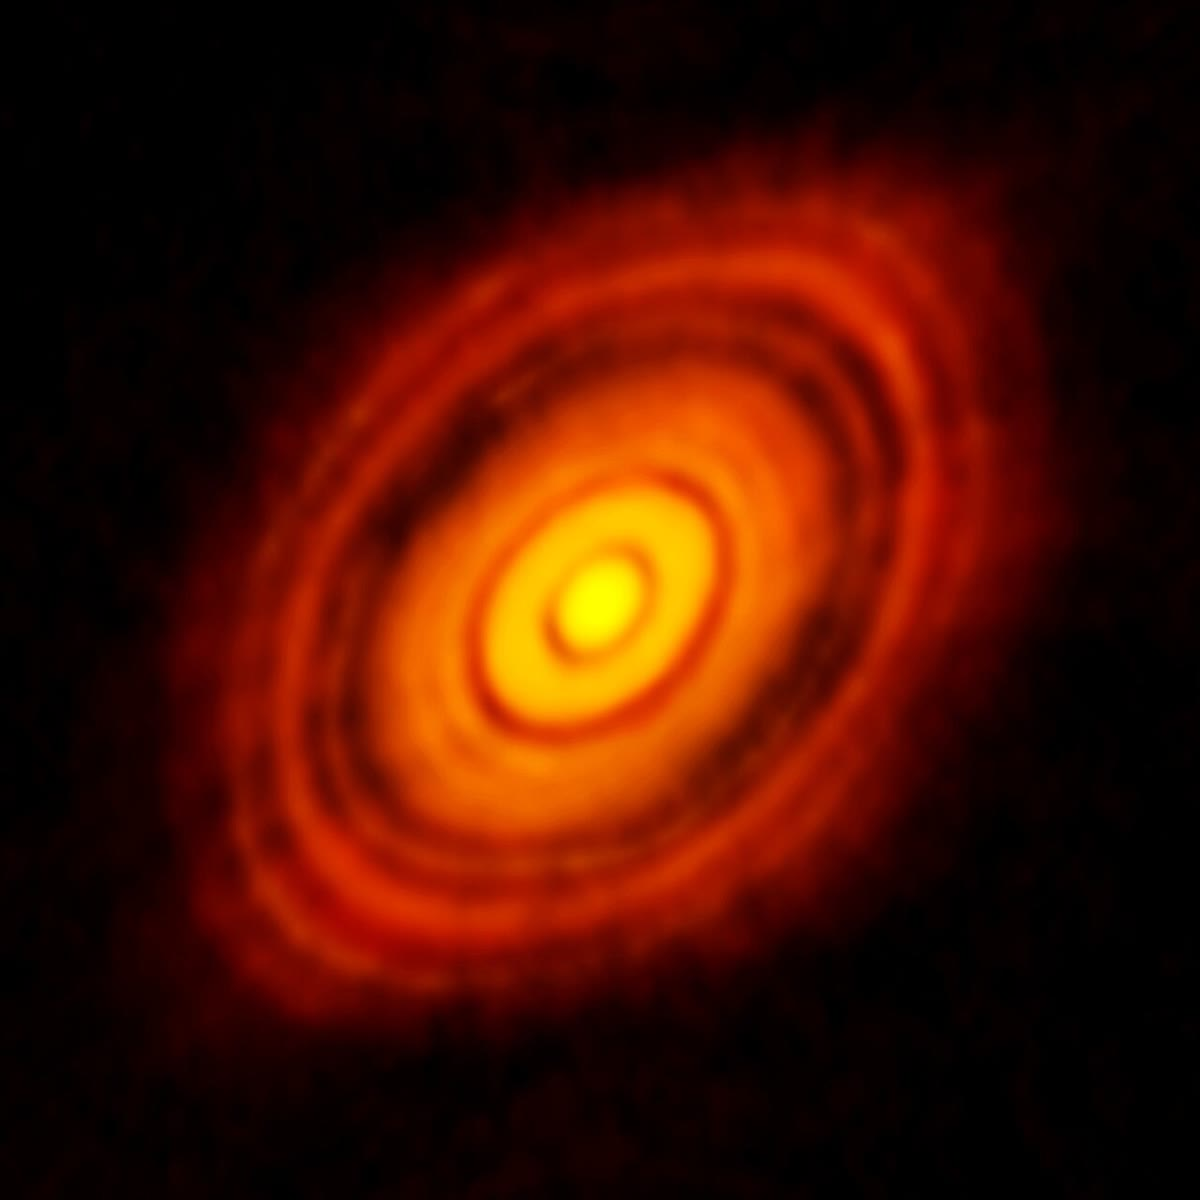
\includegraphics[width=\linewidth]{images/book4/b2-hl-tau-alma.jpg}
\end{minipage}\hfill
\begin{minipage}[c]{0.52\linewidth}
{\small El disco de la estrella joven HL Tauri, a \qty{140}{pc} en Tauro, fotografiado
por el interferómetro ALMA a una longitud de onda de cerca de un milímetro, donde brilla el polvo
frío. El disco, de unas \qty{120}{au} de radio y visto inclinado
\ang{47}, muestra anillos brillantes y oscuros de unas pocas unidades astronómicas de anchura; el
sistema tiene como mucho uno o dos millones de años, y los anillos se interpretan como los
primeros indicios de planetas que despejan su camino. ALMA (ESO/NAOJ/NRAO), CC BY 4.0.}
\end{minipage}
% ledger: alma:hltau
\end{omfigure}

El disco lo calienta la estrella. Un grano a la distancia $r$ absorbe luz estelar
sobre su sección transversal y radia por toda su superficie.

\begin{proposition}[Temperatura de un grano iluminado por una estrella]
\label{prop:b2:ism-star-formation:grain}
Un grano pequeño que se comporta como un cuerpo negro, a la distancia $r$ de una estrella de
luminosidad $L$ e iluminado por un solo lado, se estabiliza a la temperatura
\[
  T = \left(\frac{L}{16\pi\sigma r^2}\right)^{1/4},
\]
que disminuye como $r^{-1/2}$.
\end{proposition}

\begin{proof}
Un grano esférico de radio $a$ intercepta la potencia $\pi a^2\,L/(4\pi r^2)$
y, a la temperatura $T$, radia $4\pi a^2\sigma T^4$ por su superficie.
En el equilibrio ambas son iguales: $T^4 = L/(16\pi\sigma r^2)$; $a$ se simplifica.
\end{proof}

A \qty{1}{au} de una estrella como el Sol el grano está a \qty{278}{K}; a
\qty{5.2}{au}, donde orbita Júpiter, a \qty{122}{K}. El hielo de agua se condensa donde
los granos están por debajo de unos \qty{180}{K} (las temperaturas de condensación son
las del \cref{ch:b2:planet-formation-meteorites}), es decir más allá de unas
\qty{2.4}{au}: el primer indicio de la frontera, la línea de nieve, que separa los
planetas rocosos de los helados. Un disco real es opaco, y su plano medio está protegido de la luz estelar directa; la
proposición da el orden de magnitud correcto y la pendiente correcta para las
capas superficiales que ve la estrella.
% ledger: lodders:tc-table

Los discos no duran. El exceso infrarrojo, el brillo del polvo templado por encima de lo que la estrella
sola emitiría, revela si una estrella conserva todavía un disco. Contar las estrellas
con ese exceso en cúmulos de distintas edades da la fracción de estrellas
que conservan su disco en función del tiempo (figura siguiente): la mayoría de las estrellas tienen uno
al nacer, la mitad lo han perdido hacia los tres millones de años, y casi ninguna
lo conserva más allá de seis. Los gigantes gaseosos, que deben reunir su gas del disco,
tienen que formarse en esos pocos millones de años.
% ledger: haisch:disc-fractions, haisch:disc-lifetime

\begin{omfigure}
\begin{tikzpicture}
\begin{axis}[omrecord, width=0.8\linewidth, height=5.6cm, xmin=0, xmax=8.5, ymin=0, ymax=1.05,
  xlabel={edad del cúmulo (Myr)}, ylabel={fracción de estrellas con disco},
  tick label style={font=\scriptsize}, label style={font=\small}, clip=false]
\addplot[thick, black!55, densely dashed] table[x=age, y=frac] {figdata/out/bachelor-2-jeans-discfit.dat};
\addplot[only marks, mark=*, mark size=1.8pt, blue!70!black,
  error bars/.cd, y dir=both, y explicit]
  table[x=age, y=frac, y error=err, restrict x to domain=0:10] {figdata/out/bachelor-2-jeans-discs.dat};
\node[font=\scriptsize, anchor=north west] at (axis cs:0.05,0.74) {NGC 2024};
\node[font=\scriptsize, anchor=south west] at (axis cs:1.55,0.86) {Trapecio};
\node[font=\scriptsize, anchor=south west] at (axis cs:2.35,0.71) {IC 348};
\node[font=\scriptsize, anchor=south west] at (axis cs:3.3,0.56) {NGC 2264};
\node[font=\scriptsize, anchor=south west] at (axis cs:5.1,0.15) {NGC 2362};
\node[font=\scriptsize, anchor=north east] at (axis cs:8.4,0.98) {(NGC 1960, \qty{30}{Myr}: $0.03$)};
\end{axis}
\end{tikzpicture}

\par\smallskip{\small Fracción de las estrellas de cúmulos jóvenes que muestran el exceso
infrarrojo de un disco, frente a la edad del cúmulo (con su error), según Haisch, Lada
y Lada (2001). La línea discontinua es la recta de mínimos cuadrados que pasa por los cinco
cúmulos más jóvenes: llega a $0.5$ a los \qty{3.0}{Myr} y a cero a los \qty{6.1}{Myr}
(\cref{exo:b2:ism-star-formation:12}).}
\end{omfigure}

\begin{inthelab}[Ver a través del polvo con ondas de radio]
\begin{minipage}[t]{0.55\linewidth}\vspace{0pt}
El gas y el polvo fríos son invisibles para los telescopios ópticos pero brillan en longitudes
de onda milimétricas, donde la atmósfera solo es transparente sobre lugares altos y secos. Una
antena de radio del tamaño de una casa resuelve poco a esas longitudes de onda, así que los
astrónomos combinan muchas: en un interferómetro cada par de antenas, separadas
por una línea de base, mide una componente del patrón de brillo del cielo, y
un ordenador reconstruye la imagen a partir de los cientos de pares que forman unas treinta antenas. La resolución es la de
un único telescopio tan ancho como la línea de base más larga: con antenas repartidas sobre
\qty{15}{km}, el disco de HL Tauri se fotografió con detalles de unas pocas unidades astronómicas a
\qty{140}{pc}. Los operadores trasladan las antenas en transportadores entre configuraciones,
y el correlador combina sus señales en tiempo real.
\end{minipage}\hfill
\begin{minipage}[t]{0.42\linewidth}\vspace{0pt}
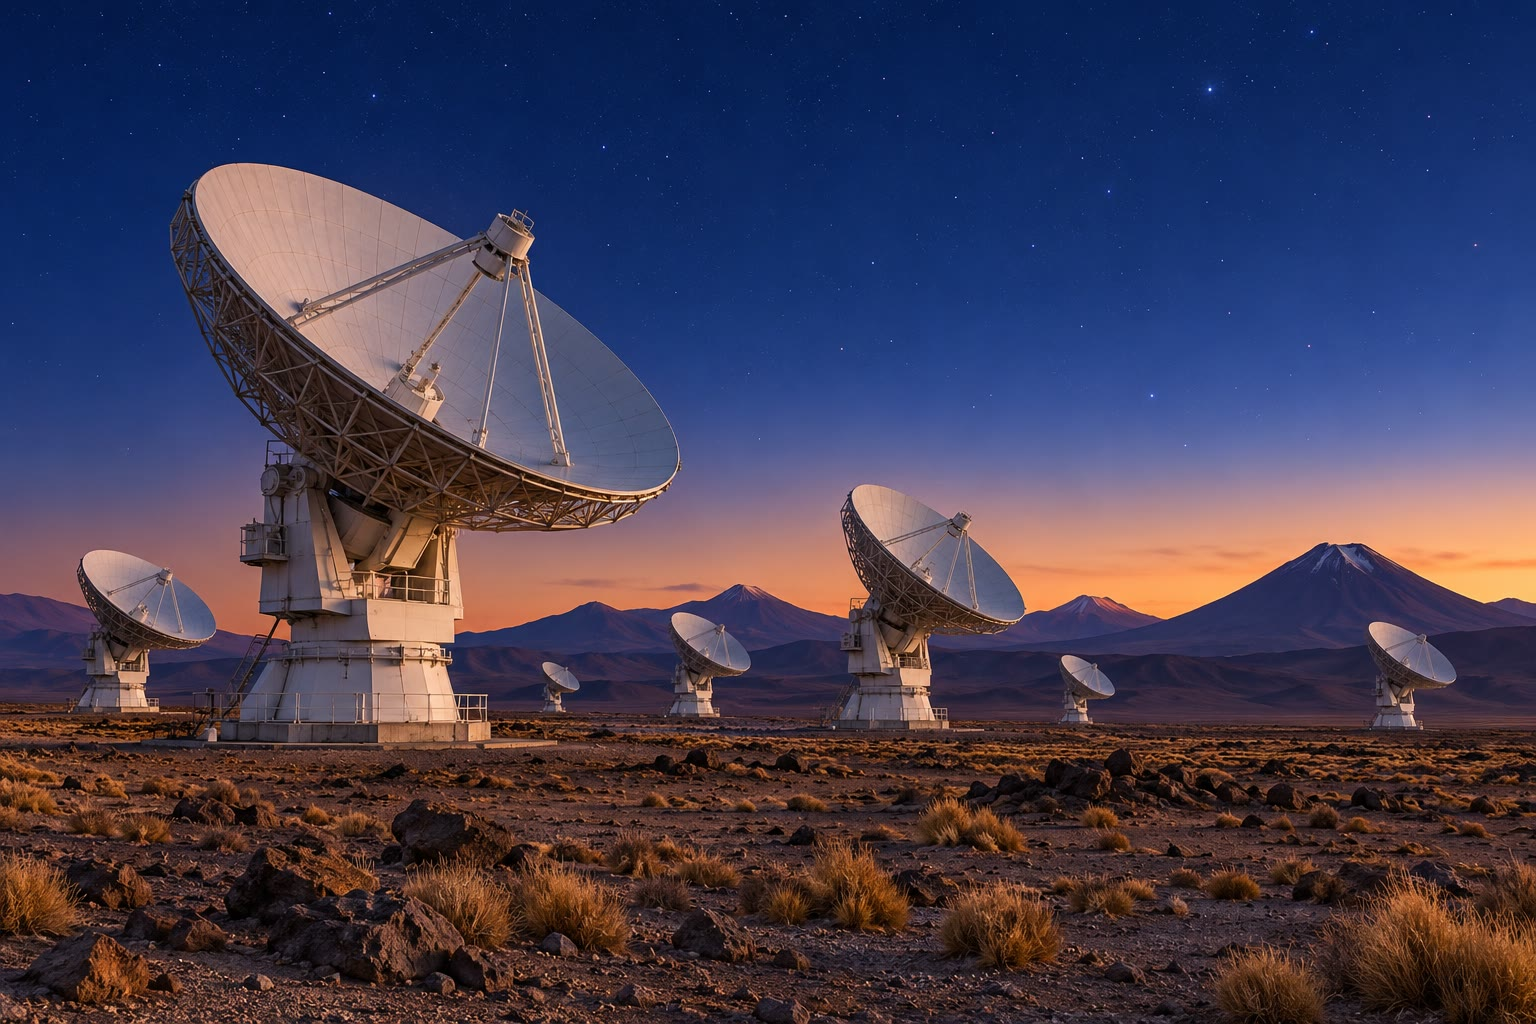
\includegraphics[width=\linewidth]{images/book4/ai/b2-radio-array.jpg}

{\scriptsize Una red de antenas de radio en una alta meseta desértica al atardecer
(ilustración generada por IA).}
\end{minipage}
% ledger: alma:hltau, alma:baselines
\end{inthelab}

\section{Ejercicios}

\begin{exercise}[$\star$]\label{exo:b2:ism-star-formation:1}
La densidad interestelar media cerca del Sol es \qty{2.7e-24}{g.cm^{-3}}. Tomando
la masa de un átomo de hidrógeno como \qty{1.67e-24}{g}, calcúlese el número de átomos de
hidrógeno por centímetro cúbico. Compárese con el número de moléculas por centímetro
cúbico en el aire a \qty{101325}{Pa} y \qty{288}{K} ($n = P/k_{\mathrm B}T$).
% ledger: ferriere:mean-density, const:kB
\end{exercise}

\begin{exercise}[$\star$]\label{exo:b2:ism-star-formation:2}
Con el valor $M_J = 5.46$ masas solares a \qty{10}{K} y $10^4$ partículas
por centímetro cúbico, y la dependencia de $M_J$ con la densidad, calcúlese la \omterm{def:b2:ism-star-formation:jeans}{masa de
Jeans} a \qty{10}{K} y $10^2$ partículas por centímetro cúbico. ¿Cuántas \omterm{def:b2:ism-star-formation:jeans}{masas de
Jeans} contiene la nube de Tauro, de \num{24000} masas solares?
% ledger: goldsmith:taurus-mass
\end{exercise}

\begin{exercise}[$\star$]\label{exo:b2:ism-star-formation:3}
Calcúlese la velocidad isoterma del sonido $c_s = (k_{\mathrm B}T/\mu m_u)^{1/2}$ del
gas molecular ($\mu = 2.33$, $m_u = \qty{1.661e-27}{kg}$) a \qty{10}{K} y a
\qty{100}{K}. ¿Cuánto tarda una onda sonora en atravesar un núcleo de radio
\qty{0.1}{pc} a \qty{10}{K}, en millones de años?
% ledger: kauffmann:mu, nist:u, iau:parsec
\end{exercise}

\begin{exercise}[$\star$]\label{exo:b2:ism-star-formation:4}
Calcúlese el \omterm{def:b2:ism-star-formation:free-fall}{tiempo de caída libre} de un \omterm{def:b2:ism-star-formation:molecular-cloud}{núcleo denso} de $10^5$ partículas por centímetro
cúbico y de una nube oscura de $10^2$ ($\mu = 2.33$). ¿Cuál colapsa
más deprisa, y en qué factor?
\end{exercise}

\begin{exercise}[$\star\star$]\label{exo:b2:ism-star-formation:5}
Demuéstrese que $M_J$ puede escribirse $M_J = 5^{3/2}\,(3/4\pi)^{1/2}\,c_s^3\,G^{-3/2}\rho^{-1/2}$.
A temperatura fija, ¿en qué factor debe aumentar la densidad de un núcleo para reducir a la mitad
su \omterm{def:b2:ism-star-formation:jeans}{masa de Jeans}? A densidad fija, ¿en qué factor cambia la \omterm{def:b2:ism-star-formation:jeans}{masa de Jeans} si
el núcleo se calienta de \qty{10}{K} a \qty{20}{K}?
\end{exercise}

\begin{exercise}[$\star\star$]\label{exo:b2:ism-star-formation:6}
Una estrella joven tiene la masa del Sol, el doble de su radio y el doble de su luminosidad
($M_\odot = \qty{1.989e30}{kg}$, $R_\odot = \qty{6.96e8}{m}$,
$L_\odot = \qty{3.83e26}{W}$). Calcúlese su tiempo de Kelvin--Helmholtz en millones de
años, y compárese con la duración de los discos.
% ledger: sun:mass, sun:R, sun:L
\end{exercise}

\begin{exercise}[$\star\star$]\label{exo:b2:ism-star-formation:7}
Calcúlese la tasa de acreción $c_s^3/G$ de una \omterm{def:b2:ism-star-formation:protostar}{protoestrella} en un núcleo a \qty{10}{K}, en
masas solares por año, y el tiempo que tarda en reunir una masa solar. Las mismas
preguntas para un núcleo a \qty{20}{K}.
\end{exercise}

\begin{exercise}[$\star\star$]\label{exo:b2:ism-star-formation:8}
Con la \cref{prop:b2:ism-star-formation:grain} y $L_\odot = \qty{3.83e26}{W}$,
calcúlese la distancia al Sol, en unidades astronómicas, a la que un grano
alcanza \qty{1300}{K}, cerca de la temperatura a la que condensan los silicatos comunes
(\cref{ch:b2:planet-formation-meteorites}), y
la temperatura de un grano a la distancia de Júpiter, \qty{5.2}{au}.
% ledger: sun:L, const:sigma, const:au
\end{exercise}

\begin{exercise}[$\star\star$]\label{exo:b2:ism-star-formation:9}
El gas del disco de HL Tauri gira alrededor de una estrella de unas \num{1.3} masas
solares. Calcúlense la velocidad kepleriana y el periodo orbital a \qty{100}{au}.
Si el sistema tiene un millón de años, ¿cuántas vueltas ha dado el gas a
\qty{100}{au} desde que se formó la estrella?
% ledger: alma:hltau
\end{exercise}

\begin{exercise}[$\star\star\star$]\label{exo:b2:ism-star-formation:10}
Hállese la energía gravitatoria de una esfera de radio $R$ en la que la densidad
disminuye como $\rho(r) = \rho_0 R/r$, y compárese con la de una esfera uniforme de
la misma masa y el mismo radio. Concentrar la masa hacia el centro, ¿hace
la nube más fácil o más difícil de sostener por su energía térmica?
\end{exercise}

\begin{exercise}[$\star\star\star$]\label{exo:b2:ism-star-formation:11}
Un núcleo de radio \qty{0.1}{pc} gira como un sólido rígido con la velocidad angular
$\Omega = \qty{1e-14}{rad.s^{-1}}$. Calcúlense su periodo de rotación, el momento angular
específico $j = \Omega R^2$ del gas en su ecuador y el radio
centrífugo de ese gas alrededor de una estrella de una masa solar, en unidades astronómicas.
¿Por qué el gas del interior del núcleo cae más cerca de la estrella?
\end{exercise}

\begin{exercise}[$\star\star\star$]\label{exo:b2:ism-star-formation:12}
Las fracciones de discos de los cinco cúmulos más jóvenes de la figura de la última
sección son $0.85$, $0.80$, $0.65$, $0.52$ y $0.12$ a 0.3, 1.5, 2.3, 3.2 y
\qty{5.0}{Myr}. Ajústese a mano una recta de mínimos cuadrados $f = a - bt$
(calcúlense las medias, y después $\sum(t - \bar t)(f - \bar f)$ y
$\sum(t - \bar t)^2$). ¿A qué edad llega a un medio, y a cero? ¿Por qué una
recta es un mal modelo más allá de esa edad?
% ledger: haisch:disc-fractions
\end{exercise}

\section{Problema: un núcleo en la nube de Aldra}

\begin{problem}[{Problema de fin de semana --- la masa y la estabilidad de un núcleo denso leídas en un
mapa de polvo, el nacimiento de su protoestrella y el tamaño de su disco}]
\label{pb:b2:ism-star-formation:1}
% values: calc/ch01.py
% ledger: kauffmann:mu, nist:u, iau:parsec, const:G, const:kB, sun:mass, sun:R, sun:L, const:au, const:sigma, bt07:cores, alma:hltau
La nube de Aldra es una nube oscura inventada. Un mapa milimétrico de su polvo
muestra un núcleo redondo de radio \qty{0.08}{pc}, con una densidad de columna media de
$N(\ce{H2}) = \num{1.5e22}$ moléculas de hidrógeno por centímetro cuadrado. Una
línea del amoniaco da la temperatura del gas, \qty{10}{K}, y un gradiente de
velocidad de \qty{0.4}{km.s^{-1}} por pársec a través del núcleo, interpretado como rotación
de sólido rígido. Úsense $G = \qty{6.674e-11}{m^3.kg^{-1}.s^{-2}}$,
$k_{\mathrm B} = \qty{1.381e-23}{J.K^{-1}}$, $m_u = \qty{1.661e-27}{kg}$,
\qty{1}{pc} $= \qty{3.086e16}{m}$, \qty{1}{au} $= \qty{1.496e11}{m}$, un año de
\qty{3.156e7}{s}, $M_\odot = \qty{1.989e30}{kg}$, $R_\odot = \qty{6.96e8}{m}$,
$L_\odot = \qty{3.83e26}{W}$, $\sigma = \qty{5.67e-8}{W.m^{-2}.K^{-4}}$; la
masa por molécula de hidrógeno, helio incluido, es $2.8\,m_u$, y la masa media
por partícula $2.33\,m_u$.

\medskip
\noindent\textbf{Parte I --- Masa y densidad.}
\begin{enumerate}
  \item Conviértase el radio del núcleo a metros.
  \item Calcúlese la masa por metro cuadrado de la columna, $2.8\,m_u N$.
  \item Dedúzcase la masa del núcleo, en kilogramos y en masas solares.
  \item Calcúlense su volumen y su densidad media.
  \item Calcúlese el número de partículas por centímetro cúbico.
  \item ¿Es un \omterm{def:b2:ism-star-formation:molecular-cloud}{núcleo denso} en el sentido de la tabla de la segunda sección?
\end{enumerate}

\noindent\textbf{Parte II --- Estabilidad.}
\begin{enumerate}[resume]
  \item Calcúlese la \omterm{def:b2:ism-star-formation:jeans}{masa de Jeans} del gas del núcleo, en masas solares.
  \item ¿Cuántas \omterm{def:b2:ism-star-formation:jeans}{masas de Jeans} contiene el núcleo? ¿Es estable?
  \item Calcúlese la \omterm{def:b2:ism-star-formation:jeans}{longitud de Jeans} y compárese con el radio del núcleo.
  \item ¿Cuál sería la \omterm{def:b2:ism-star-formation:jeans}{masa de Jeans} si el gas estuviera a \qty{20}{K}? ¿Seguiría
        colapsando el núcleo?
  \item Calcúlese el \omterm{def:b2:ism-star-formation:free-fall}{tiempo de caída libre} del núcleo, en miles de años.
  \item Compárese con el tiempo que tarda una onda sonora en atravesar el núcleo. ¿Qué
        proceso es más rápido, y qué significa eso?
\end{enumerate}

\noindent\textbf{Parte III --- La protoestrella.}
\begin{enumerate}[resume]
  \item Calcúlese la velocidad del sonido en el núcleo.
  \item Calcúlese la tasa de acreción $c_s^3/G$, en masas solares por año.
  \item Calcúlese el tiempo necesario para reunir una masa solar a este ritmo.
  \item Si un tercio del núcleo acaba en estrellas, ¿cuántas estrellas de una masa solar
        puede formar?
  \item Agotada la envoltura, la estrella tiene una masa solar, tres radios
        solares y cuatro luminosidades solares. Calcúlese su tiempo de Kelvin--Helmholtz.
  \item ¿Es más largo o más corto que el tiempo de acreción? ¿Qué tipo de estrella es
        entonces?
\end{enumerate}

\noindent\textbf{Parte IV --- El disco.}
\begin{enumerate}[resume]
  \item Conviértase el gradiente de velocidad en una velocidad angular $\Omega$, en
        \unit{rad.s^{-1}}.
  \item Calcúlese el momento angular específico $j = \Omega R^2$ del gas en el
        ecuador del núcleo.
  \item Calcúlese su radio centrífugo alrededor de una estrella de una masa solar, en
        unidades astronómicas.
  \item Calcúlese la temperatura de un grano a \qty{1}{au} y a \qty{30}{au}
        de una estrella de una luminosidad solar.
  \item ¿Dónde está la línea de nieve de este disco, si el hielo de agua sobrevive por debajo de
        \qty{180}{K}?
  \item Indíquese el tiempo necesario para ensamblar la estrella de la pregunta 15, la cifra
        clave de este problema, en miles de años, y compárese con el
        \omterm{def:b2:ism-star-formation:free-fall}{tiempo de caída libre} de la pregunta 11.
\end{enumerate}
\end{problem}
